% !TeX root = ../Book1.tex
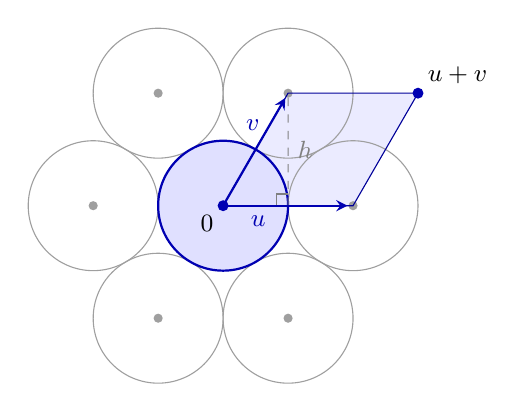
\begin{tikzpicture}[>=stealth,font=\small,scale=1.65]
	\pgfmathsetmacro{\triheight}{sqrt(3)/2}
	\coordinate (O) at (0,0);
	\coordinate (U) at (1,0);
	\coordinate (V) at (.5,\triheight);
	\coordinate (W) at (1.5,\triheight);
	\fill[blue!8] (O)--(U)--(W)--(V)--cycle;
	\fill[blue!12] (O) circle[radius=.5];
	\foreach \ang in {0,60,120,180,240,300} {
		\draw[gray!75] (\ang:1) circle[radius=.5];
		\fill[gray!75] (\ang:1) circle[radius=1pt];
	}
	\draw[blue!70!black,thick] (O) circle[radius=.5];
	\draw[blue!60!black] (O)--(U)--(W)--(V)--cycle;
	\draw[gray,dashed] (.5,0)--(V) node[midway,right] {\(h\)};
	\draw[gray] (.5,.09)--(.41,.09)--(.41,0);
	\draw[->,thick,blue!70!black,shorten >=2pt] (O)--(U) node[pos=.27,below] {\(u\)};
	\draw[->,thick,blue!70!black,shorten >=2pt] (O)--(V) node[pos=.72,left] {\(v\)};
	\fill[blue!70!black] (O) circle[radius=1.2pt];
	\fill[blue!70!black] (W) circle[radius=1.2pt];
	\node[below left] at (O) {\(0\)};
	\node[above right] at (W) {\(u+v\)};
\end{tikzpicture}
